\documentclass{article}

\usepackage{float}
\usepackage{hyperref}
\usepackage{tabularx}
\usepackage{graphicx}


\usepackage{listings}
\lstset{
basicstyle=\small\ttfamily,
columns=flexible,
breaklines=true
}

\title{Motion Controller and Odometry Interface for the RCV}
\author{Lars Svensson \& Rui Oliveira}
\date{February 2016}


\begin{document}
  
  
\maketitle

Develop a useful and easy to use interface that will allow the RCV to be used reliably and easily through ROS. A simple diagram of the expected outcome is as follows:


\begin{figure}[h!]
\centering
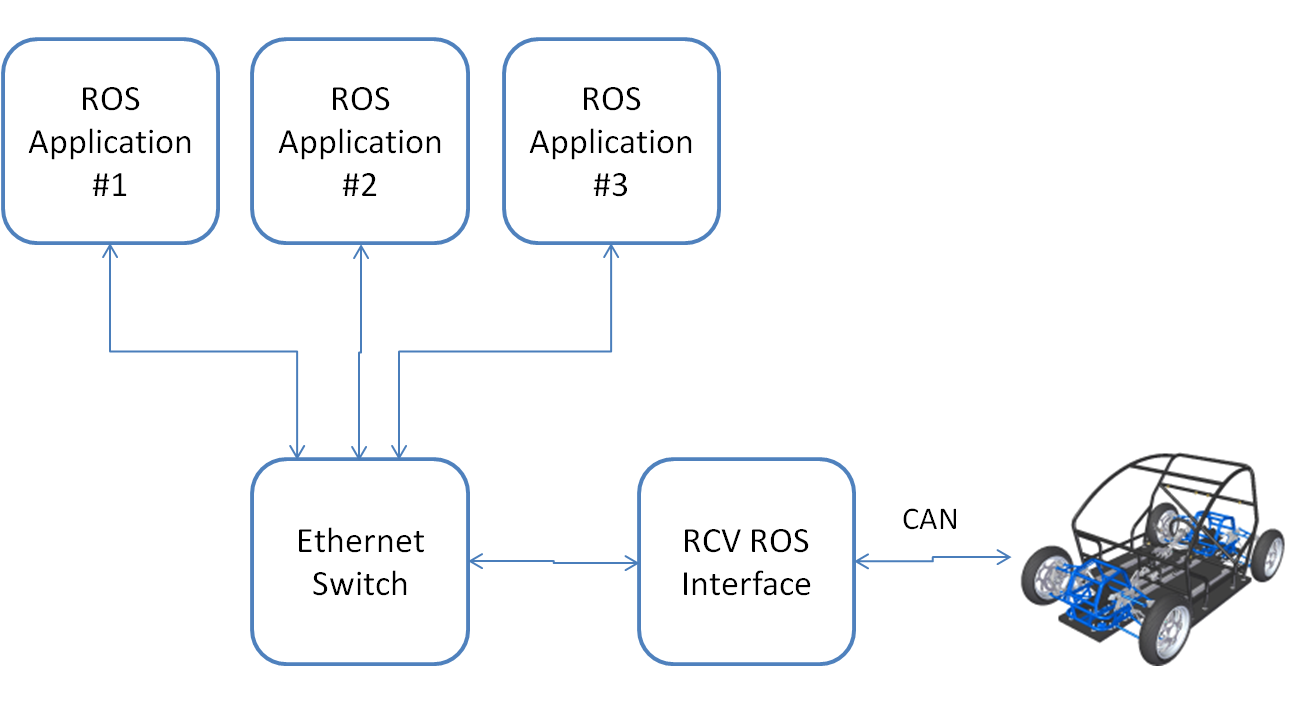
\includegraphics[width=1.0\textwidth]{systemStructure2.png}
\caption{System Structure Draft}
\label{fig:systemStructure}
\end{figure} 


There are many aspects that can be developed in the RCV, however it is necessary to choose only those which are required for the correct usage of the RCV by the other parties interested. Several functionalities will be described in this proposal, and they will be divided into Mandatory and Optional functionalities. The division made is based on a first thought of the authors on what might be, or not, required from the other students. It is not a final decision, as it might still be changed upon request from the other course participants.

An important point to make is that the Velodyne sensors are not a concern of this work. They should be easy to interface with by making use of Andreas' work.

\section{Mandatory Objectives}

\subsection{Path Following Controller}

The Path Following Controller will be able to receive path requests and will be responsible for following them. The paths will be sent to the controller in a fixed reference frame, as displayed in figure \ref{fig:fixedReferential}, for example UTM coordinates. The path may be updated at a fixed rate or at irregular intervals, provided that the the updated path connects with the previous one.

%\begin{figure}[h!]
%\centering
%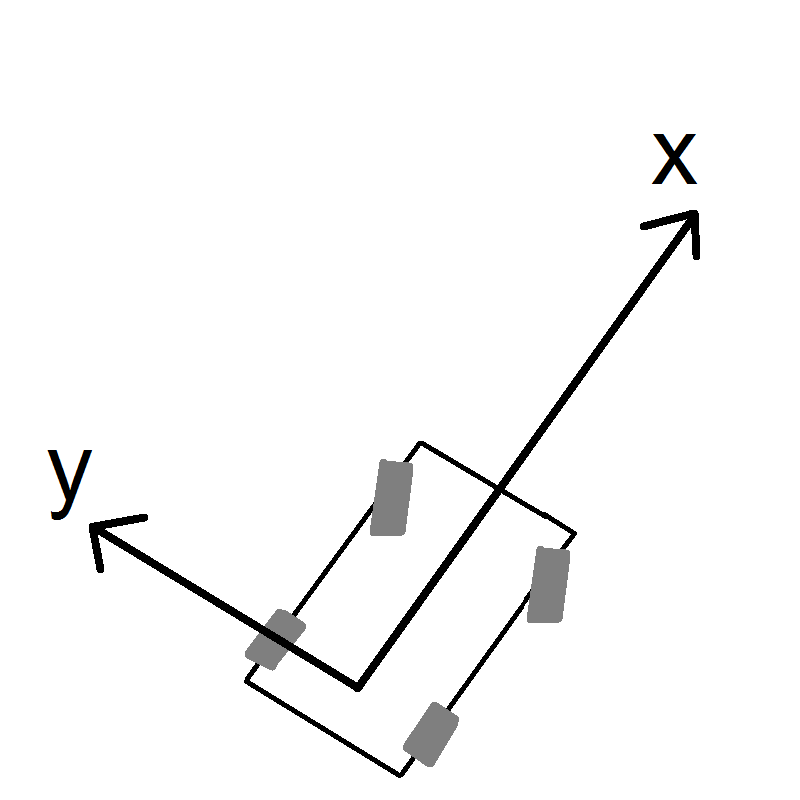
\includegraphics[width=0.7\textwidth]{localReferential}
%\caption{Local (moving) Referential}
%\label{fig:localReferential}
%\end{figure} 

\begin{figure}[h!]
\centering
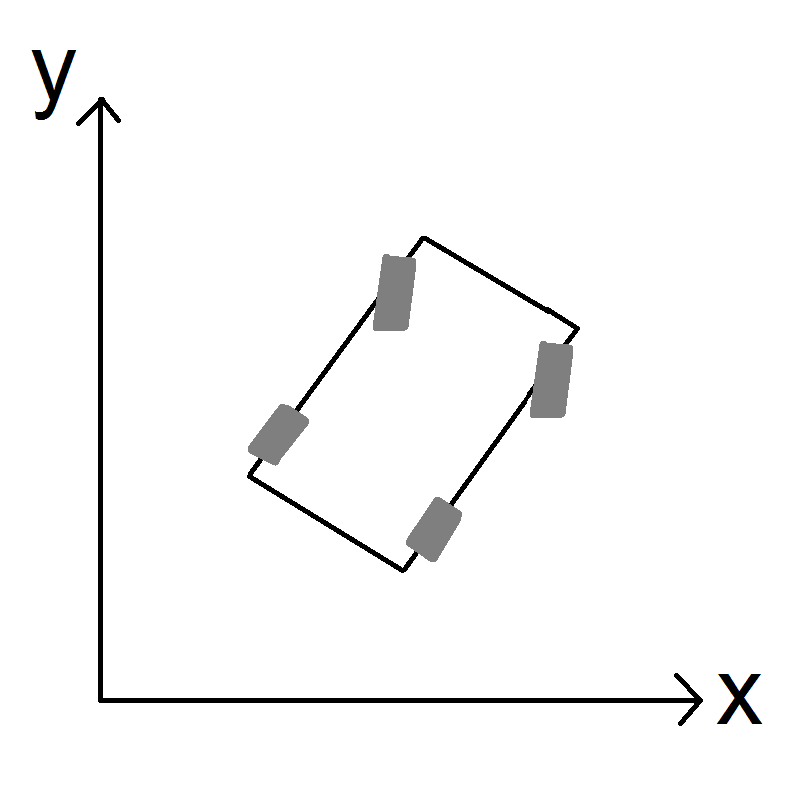
\includegraphics[width=0.7\textwidth]{fixedReferential}
\caption{Fixed Referential}
\label{fig:fixedReferential}
\end{figure} 



%In order to make the system reusable and useful for different purposes, the trajectory requests can come in the following ways:
%	An (x,y,θ) trajectory, i.e.,  a set of (x,y,θ) states with an associated time;
%	An (x,y,θ) path with a fixed velocity;
%	A GPS trajectory, with an associated time;
%	A GPS path with a fixed velocity;
%	
%\subsection{Benefits}
%
%Providing a controller that will follow given paths. Emphasys will be put in simplifying as much as possible its use. For that purpose there will be well defined interfaces, allowing the users to send commands in the way they are more comfortable with, either GPS coordinates or Cartesian coordinates. Cartesian coordinates are often a cause of trouble due to ambiguous definitions of its referentials. The system will also provide simple ways to use and define different referentials (as examples see figures \ref{fig:fixedReferential} and \ref{fig:localReferential}). 
% 


\subsection{Low Level Sensor Readings Interface}

With this task we will present the ROS user with an easy way to have access to all of the low level information of the RCV. This includes, among others, steering wheel angles, wheel encoder readings and gas pedal position.


\subsection{State Estimator Interface}
Recent Msc thesis work on the RCV includes development and implementation of a Kalman filter for state estimation. The algorithm fuses information from multiple on-board sensors into optimal (with respect to a cost function) estimates of the vehicle state. This information may be useful for higher level functionality and therefore, it will be included in the interface.

\section{Optional Objectives} 
 
%\subsection{IMU Readings Interface}
%
%This will allow the ROS user to have access to the information transmitted from the IMU.
%
%\subsection{GPS Readings Interface}
%
%This will allow the ROS user to have access to the information transmitted from the GPS.
% 
%\subsection{GPS Based Path Following}
%
%Based on the GPS measurements, the RCV will be able to follow a path defined of GPS waypoints.
 
%\subsection{Risks}
%
%Ideally the Controller will be implemented by a Master Thesis Student, if that fails, an alternative controller will have to be developed from scratch.
%Assumptions:
%The given path is feasible, otherwise the controller will safely handle it (warning and/or stopping).

\subsection{Lane Marking Camera Interface}

The RCV will soon be equipped with a Lane Detection camera from Scania. This camera is currently using CAN for message transmission. A possible ROS interface can be done such that the camera information arrives easily to computers in the Network.

\subsection{Lane Keeping Controller}

If possible (or required), a lane keeping command can also be implemented. This will make use of the Lane Tracking camera that will be implemented in the RCV. Very high level commands can then be sent to the RCV:

\begin{itemize}
\item Keep on lane with a fixed velocity or fixed acceleration
\item Change to a different lane
\item More complicated commands, such as those happening in intersections
\end{itemize}
	
%		
%	
%\subsection{Benefits}
%
%Providing a simple and robust controller to drive in well behaved (nice lane markings) roads.
%
%\subsection{Risks}
%
%The camera system still has to be tested, and its performance evaluated.

\subsection{Radar Safety Checking}

If possible a Radar will be integrated and will serve as a safety check, overriding a commanded path in case it shows a collision according to the radar measurements.

\subsection{Odometry}

A simple odometry/Information system can be implemented, it will be responsible from broadcasting general information about the car such as its position and velocities relative to a user defined frame.
Not much state estimation effort will be put into it, it will simply make use of the existing GPS/IMU to generate odometry information. 
The generated odometry will be processed and displayed in a simple way to the user, and be consistent with the desired coordinate system.

This will allow the user to define fixed frames (figure \ref{fig:fixedReferential}) and send path commands in this easier to use frame.

 
 

\subsection{Platform Health}

Typical sources of errors will be shown to the user (battery check, etc…)

\section{Learning outcomes}
The aim is that the project will give us further insights in two major areas. The first being the area of path and trajectory control of autonomous vehicles and the second being the control architecture and integration aspects concerning complex automated systems. Furthermore we hope to learn more about the subjects of the other students as well as working toward a higher level of automation of the RCV platform.
   
\end{document}